\documentclass[a4paper]{article}

\usepackage[pages=all, color=black, position={current page.south}, placement=bottom, scale=1, opacity=1, vshift=5mm]{background}
\SetBgContents{This is a basic template to start working on, will be modified to the appropriate journal later on}      % copyright

\usepackage[margin=1in]{geometry} % full-width

% AMS Packages
\usepackage{amsmath}
\usepackage{amsthm}
\usepackage{amssymb}

% Unicode
\usepackage[utf8]{inputenc}
\usepackage{hyperref}
\hypersetup{
	unicode,
%	colorlinks,
%	breaklinks,
%	urlcolor=cyan, 
%	linkcolor=blue, 
	pdfauthor={Benjamin Post},
	pdftitle={A simple article template},
	pdfsubject={A simple article template},
	pdfkeywords={article, template, simple},
	pdfproducer={LaTeX},
	pdfcreator={pdflatex}
}

% Vietnamese
%\usepackage{vntex}

% Natbib
\usepackage[sort&compress,numbers,square]{natbib}
\bibliographystyle{mplainnat}



\usepackage{graphicx, color}
\graphicspath{{fig/}}

%\usepackage[linesnumbered,ruled,vlined,commentsnumbered]{algorithm2e} % use algorithm2e for typesetting algorithms
\usepackage{algorithm, algpseudocode} % use algorithm and algorithmicx for typesetting algorithms
\usepackage{mathrsfs} % for \mathscr command


% Author info
\title{Drivers of Phytoplankton Community Variability in the Cariaco Basin, Venezuela}
\author{Benjamin Post$^{1,2}$ \and Esteban Acevedo-Trejos$^3$ \and Subhendu Chakraborty$^1$ \and Andrew Barton$^3$ \and Agostino Merico$^1$}

\date{
	$^1$Systems Ecology Group, Leibniz Centre for Tropical Marine Research (ZMT), Bremen, Germany \\ \\%
        $^2$School of Science, Constructor University, Bremen, Germany \\ \\%
	$^3$Earth Surface Process Modelling, GFZ German Research Centre for Geosciences, Potsdam, Germany\\ \\%
	$^4$Scripps Institution of Oceanography and Department of Ecology, Behavior and Evolution, University of California San Diego, La Jolla, CA, United States \\ \\[2ex]%
%	\today
corresponding author: \texttt{benjaminpost@aoop.de}
}

\begin{document}
    \maketitle
    
    \begin{abstract}
        this is the abstract
    
        
        \noindent\textbf{Keywords:} Phytoplankton, Diversity, Gradient Forest
    \end{abstract}
    
    \tableofcontents
    
    \section{Introduction}
    \label{sec:intro}
    
        \begin{itemize}

            %% Overarching theme: Stability of Ecosystem faunctions, Drivers of community change
            
            \item "The Cariaco Basin, located ...." - general hydrography/depth, etc.

            \item "The CARIACO Time Series ...." - talk about the Time Series, what they did, why

            \item "The Cariaco Basin has undergone marked shifts..." Talk about ecosystem, what has changed, reference prev literature

            \item "Here's where we come in..." Talk about how most of the analysis stopped after 2012, time series died out, but there is more data there and particularly looking at community data, we can see a return.

            \item "In this paper, we..." 
            
        \end{itemize}
    
    \section{Methods}
    \label{sec:methods}
        
        \begin{itemize}

            %% 
            
            \item Talk about the Basin shortly, then about the time series
            
            %% DATA SOURCES
            \item Niskin Bottle Dataset

            \item CTD Dataset

            \item Phytoplankton Microscopy

            \item HPLC (?)

            \item sediment traps (?)

            \item ERA 5 climate data for wind and precipitation
            
            \item AMO and MEI v.2 Climate indices

            %% METHODS
            \item Z-Scores calculation
            
            \item Clustering
    
            \item NMDS
            
            \item Gradient Forest
            
        \end{itemize}

    \section{Results}
    \label{sec:results}
    
    
            First of all, we have a map:
            
        \begin{figure}[ht]
            \centering
            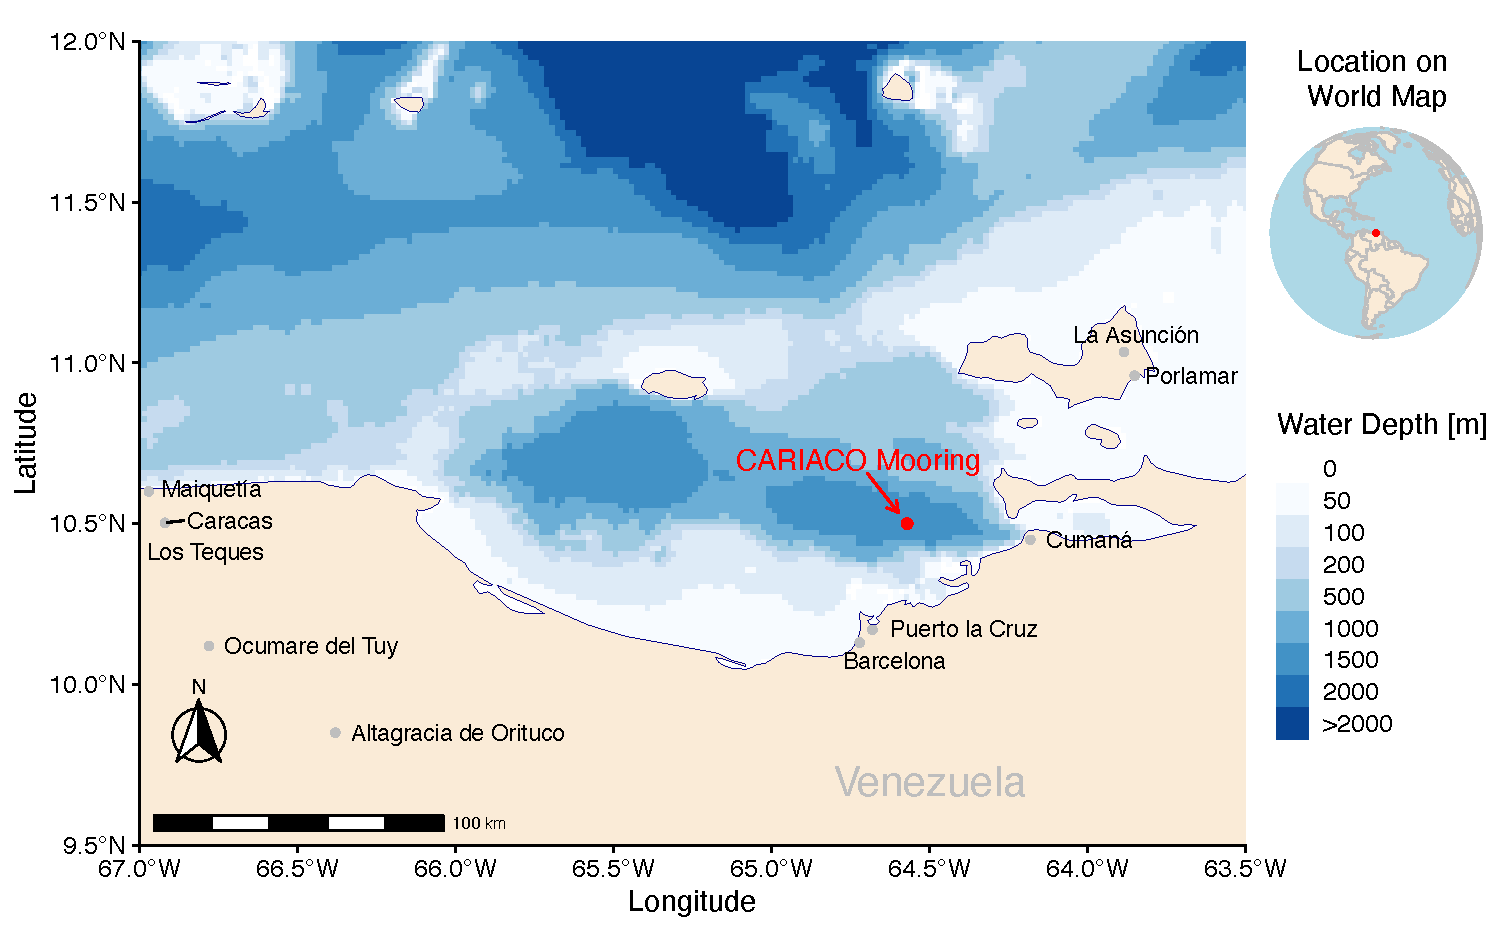
\includegraphics[width=0.7\textwidth]{fig/Artboard 1.pdf}
            \caption{Map of Location of Time Series in the Cariaco Basin, Venezuela.}
            \label{fig:example}
        \end{figure}
    
            Then we want to show some overall dynamics of the time series:
            
            \begin{figure}[ht]
            \centering
            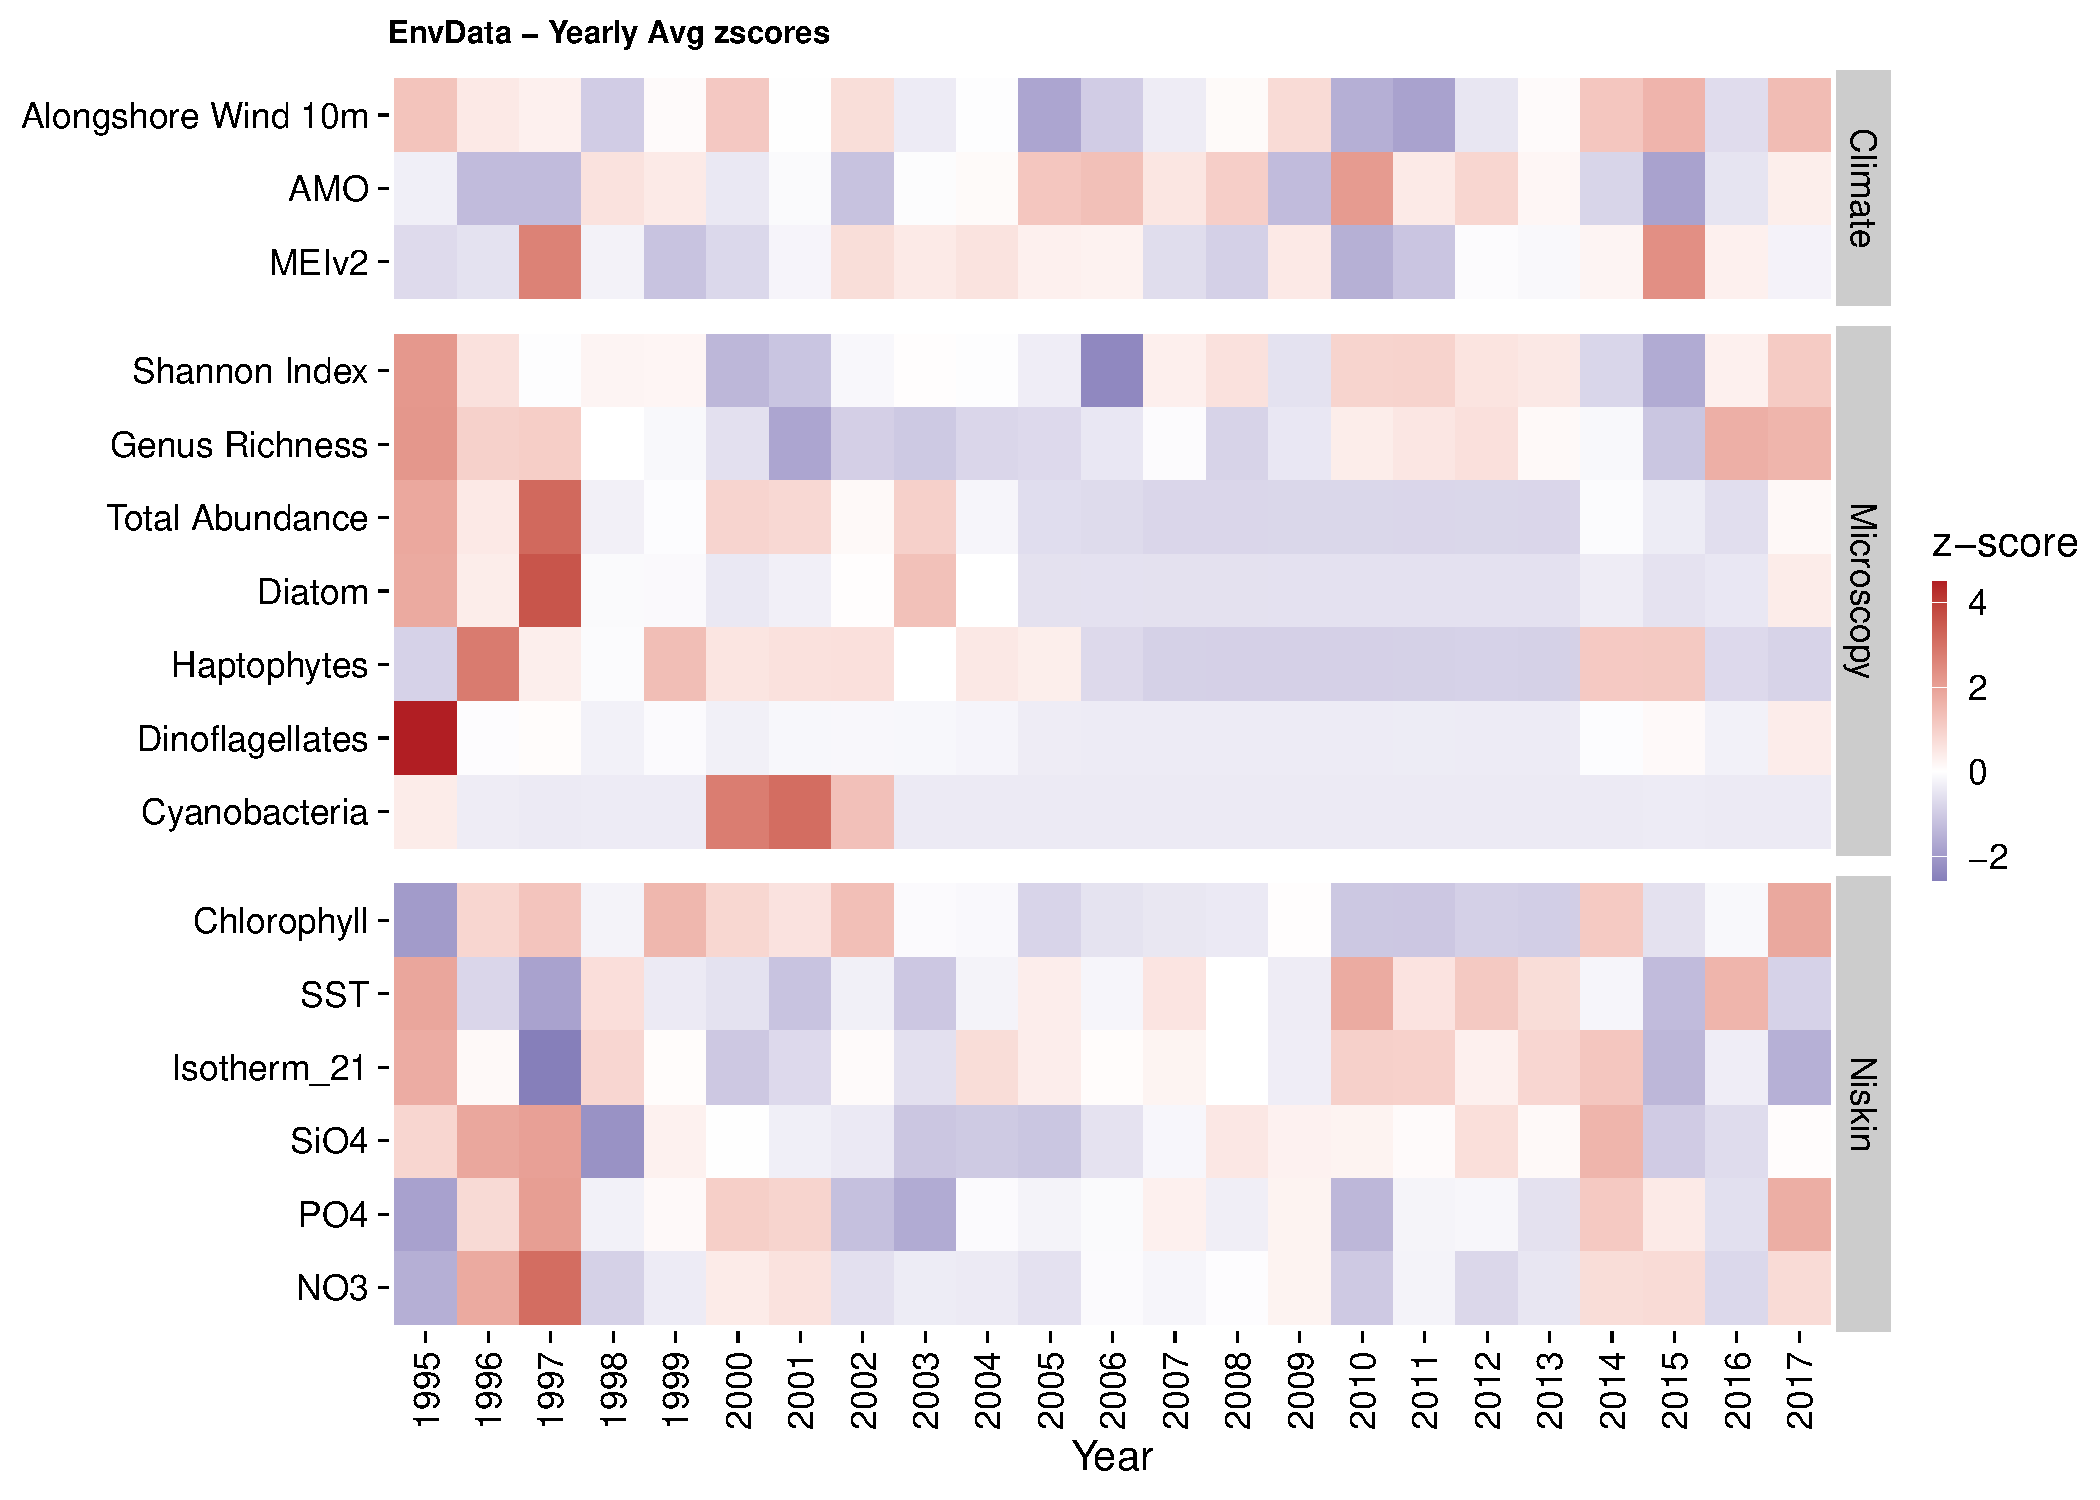
\includegraphics[width=0.7\textwidth]{fig/PLOTZScores.pdf}
            \caption{Z Scores over yearly time series..}
            \label{fig:example}
        \end{figure}
    
             Then we compare the overall dynamics with the community clustering:
            
            \begin{figure}[ht]
            \centering
            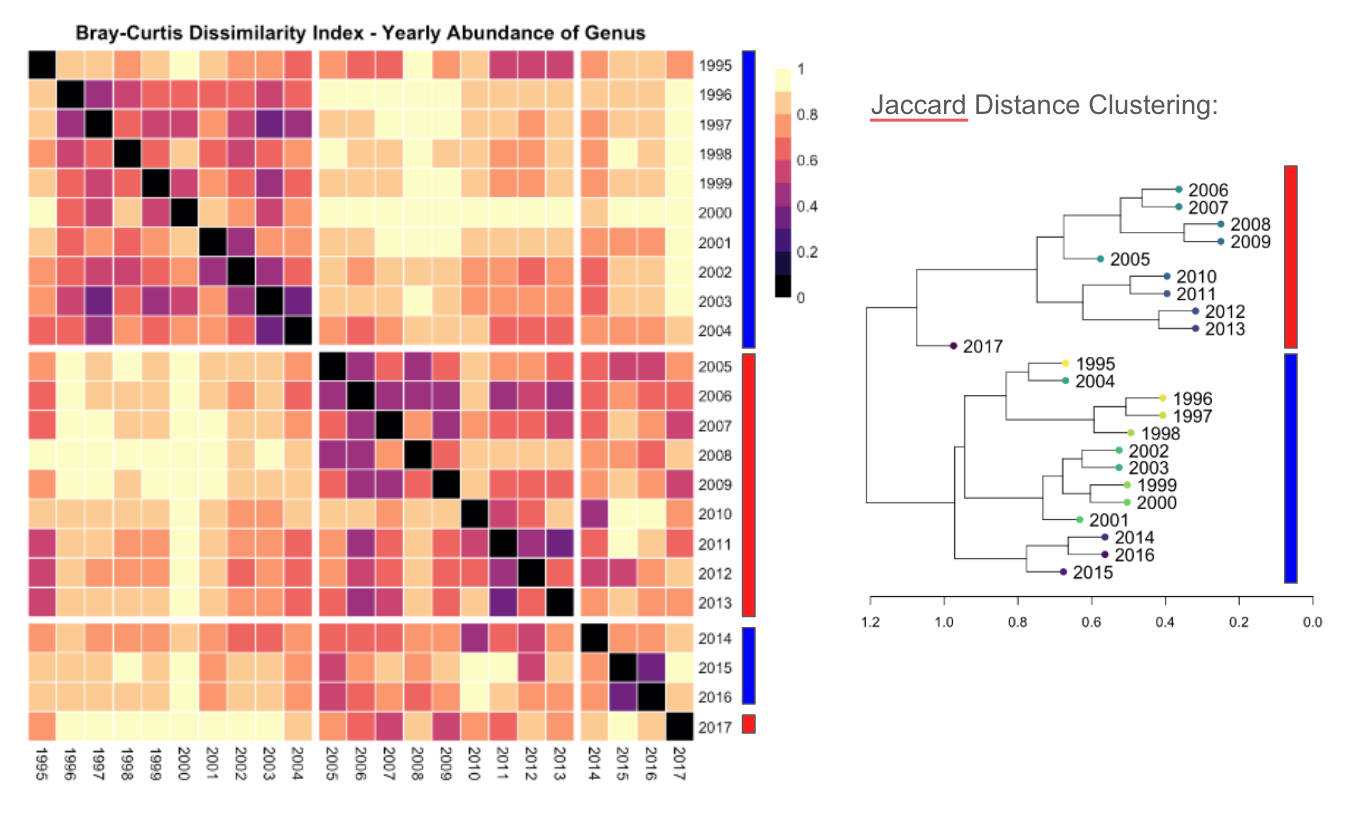
\includegraphics[width=0.7\textwidth]{fig/Screenshot 2024-08-09 at 11.10.58.png}
            \caption{Community Clustering.}
            \label{fig:example}
        \end{figure}
    
    \section{Discussion}
    \label{sec:discussion}
    
    
        \section{Conclusion}
    \label{sec:conclusion}
    
    
    
    \paragraph{Acknowledgements} Thank you to all who have helped, communicated, provided data. Claudia Benitez-Nelson, Digna Rueda-Roa, James Pinckney.
    
    %	\newpage
    \bibliography{refs}
    
    \appendix
    
    \section{Appendix 1}
    \label{app:1}
	
	
\end{document}


\textbf
	Unordered List (taken from Overleaf)
	\begin{itemize}
		\item The individual entries are indicated with a black dot, a so-called bullet.
		\item The text in the entries may be of any length.
	\end{itemize}

	Ordered List (taken from Overleaf)
	\begin{enumerate}
		\item The labels consists of sequential numbers.
		\item The numbers starts at 1 with every call to the enumerate environment.
	\end{enumerate}

	\begin{table}[ht]
		\centering
		\begin{tabular}{|c|c|}
			\hline
			\textbf{Odd} & \textbf{Even} \\
			\hline\hline
			One & Two \\
			\hline
			Three & Four \\
			\hline
		\end{tabular}
		\caption{This is a table}
		\label{tbl:1}
	\end{table}

	Table~\ref*{tbl:1} is an example of a table.
	
	\section{Discussion}
	\label{sec:examples}
	
	Now we include a figure.
	(See Figure~\ref{fig:example}.)
	\begin{figure}[ht]
		\centering
		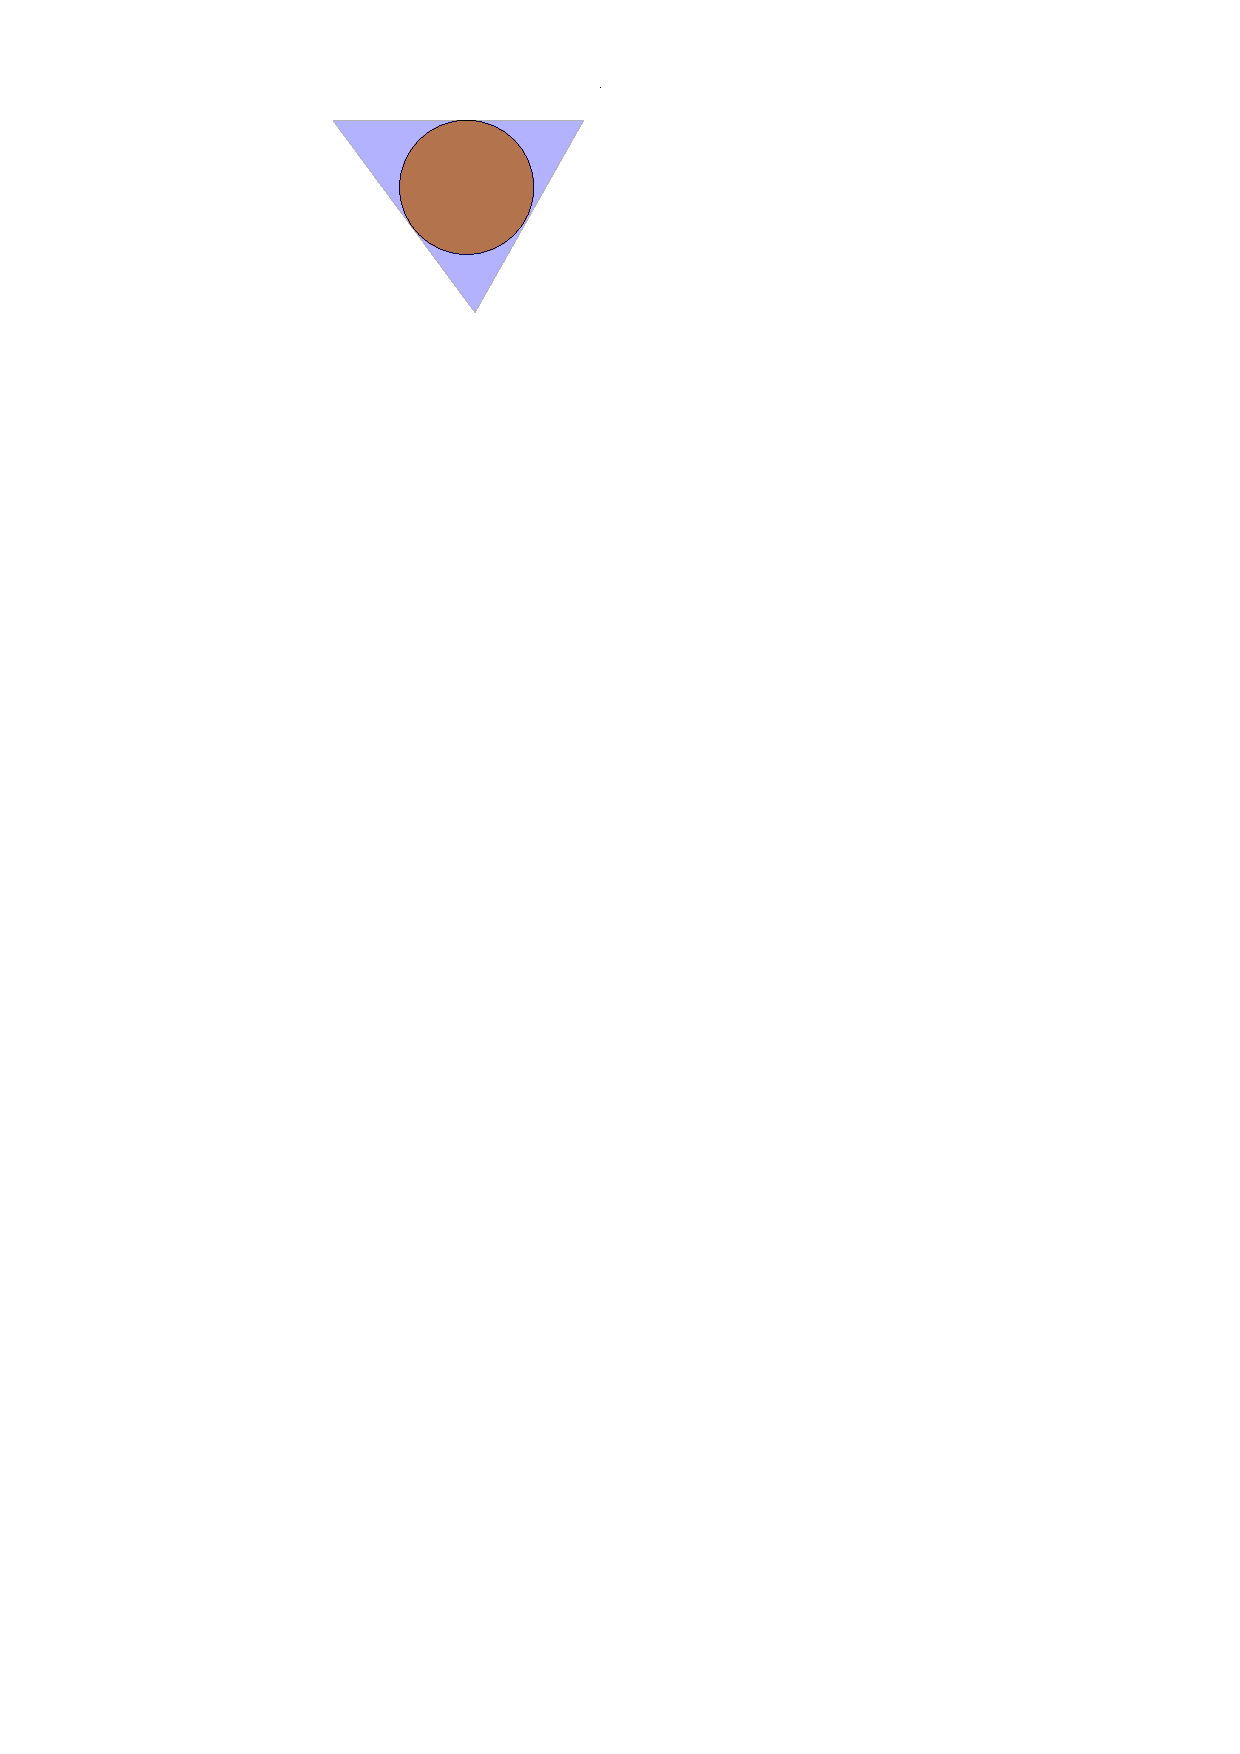
\includegraphics[width=0.3\textwidth]{example}
		\caption{An example of a figure}
		\label{fig:example}
	\end{figure}